\documentclass[12pt,fleqn]{article}\usepackage{../../common}
\begin{document}
Eğri Uydurma, Aradeğerleme (Interpolation) - 2

[4], [5], yazılarındaki konuları genişletelim. Bu yazılardan biliyoruz ki basit
regresyon

$$ y_i = \beta_0 + \beta_1 x_i + \epsilon_i$$

denklemini temel alıyor, onu veriye uyduruyor. Bu uydurma için
kullandığımız $A,x,b$ matrisleri, vektörleri var. Sihirli formülü
biliyoruz, 

$$ \hat{y} = X(X^TX)^{-1}X^Ty $$

Şimdi bu formüldeki $X$ içindeki değerleri farklı ``bazlar'' olarak görmek
faydalı olacaktır. Tek değişkenli durumda mesela bu baz

$$ X = 
\left[\begin{array}{cc}
1 & x_1 \\ \vdots & \vdots \\ 1 & x_n
\end{array}\right]
$$

Eğer karesel bir formülü uyduruyorsak, yani

$$ y_i = \beta_0 + \beta_1x_i + \beta_2x_i^2 + \epsilon_i $$

baz 

$$ X = 
\left[\begin{array}{ccc}
1 & x_1 & x_1^2\\ 
\vdots & \vdots & \vdots \\
1 & x_n & x_n^2
\end{array}\right]
$$

olur. Bu bakış açısını yorumlamak zor değil, regresyonun temeli
değişkenlerin katsayılarını bulmaktır, o zaman $1,x,x^2$ değişkenleri için
de, ya da herhangi bir başka baz bulmak için aynı teknik kullanılabilir
çünkü karesel, küpsel bazlar kullanıyor olsak bile bu değerleri önceden
hesaplayıp matrise koyduğumuz için kullandığımız sihirli formül hala lineer
bir problemi çözüyor. Hala değişkenler var, onlar bazı katsayılar ile
çarpılıp toplanarak veriye uydurulacak, ve sihirli formül bu en optimal
katsayıları bulacak.

Baz fikri ile devam edelim, alttaki veriye bakalım (gösterilen çizgilerin
daha bulunmamış olduğunu varsayalım),

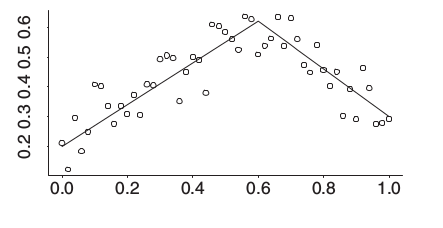
\includegraphics[width=20em]{compscieng_app20_04.png}

Bu bir kırılmış değnek (broken stick) modeli, $x=0.6$ öncesinde belli bir
eğimi olan bir düz çizgi var, sonrasında başka bir eğrisi olan bir düz
çizgi var. Kırılma noktasını biliyoruz, ya da regresyonun hangi noktadan
geçmesini istediğimizi, ilmik noktasını (knot) biliyoruz, bu durumda baz
nedir? 

$$ (x-0.6)_+$$ 

fonksiyonudur. Tanımdaki altsimge + şunu ifade eder: herhangi bir sayı $u$
eğer pozitif ise $u_+ = u$'dur, eğer değil ise $u_+ = 0$ değerine
sahiptir. Bunun amaçlarımız için mükemmel bir baz fonksiyonu olacağını
görebiliyoruz, 

$$y_i = \beta_0 + \beta_1x_i + \beta_{11}(x_i-0.6)_+ + \epsilon_i $$

Bu fonksiyonun $0.6$'ya kadar belli bir eğimi olacak, fakat $0.6$ ardından
bu eğime bir ``ek'' yapılmaya başlanacak, $\beta_{11}$ bu ekin ne kadar
olacağını yakalayacak. 

O zaman sihirli formüle verilecek matris

$$ 
X = 
\left[\begin{array}{ccc}
1 & x_1 & (x_1 - 0.6)_+ \\ 
\vdots & \vdots & \vdots \\
1 & x_n & (x_n - 0.6)_+
\end{array}\right]
$$

Regresyon çözümü bize her baz için gerekli katsayıyı (kesiyi, eğimi)
verecektir. 

Daha abartarak (!) bir sürü ilmik üzerinden bir sürü baz tanımlayabilirdik,
o zaman ufak ufak pek çok düz çizgiyi veriye uydurmak mümkün olurdu, mesela

$$ X = 
\left[\begin{array}{cccccc}
1 & x_1 & (x_1 - 0.5)_+ & (x_1 - 0.55)_+ & \dots & (x_1 - 0.96)_+\\ 
\vdots & \vdots & \vdots & \ddots & \vdots \\
1 & x_1 & (x_1 - 0.5)_+ & (x_1 - 0.55)_+ & \dots & (x_1 - 0.96)_+
\end{array}\right]
$$

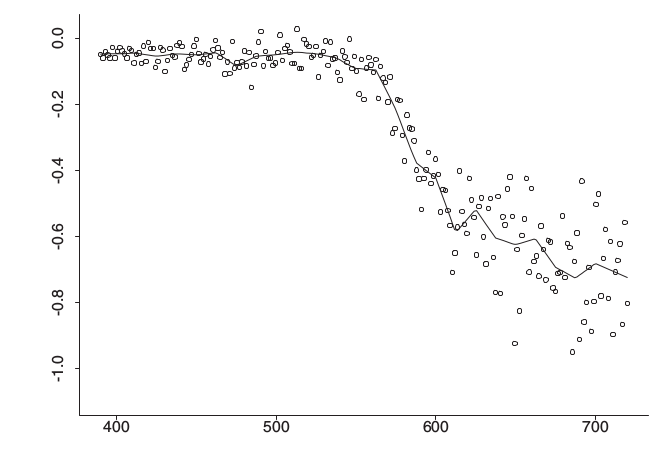
\includegraphics[width=20em]{compscieng_app20_05.png}

(Resimde ilmikler 400,500,.. gibi değerlerde, yani bazlar $(x_1-500)_+$
şeklinde olurdu)

Bilinen tek ilmik üzerinden en basit örneği görelim,

\begin{minted}[fontsize=\footnotesize]{python}
import statsmodels.formula.api as smf
import pandas as pd

df = pd.read_csv('../../tser/tser_chgpt/2inclines.csv')
reslin = smf.ols('y ~ 1 + x + I((x-55)*(x>55))', data=df).fit()
print reslin.summary()
\end{minted}

\begin{verbatim}
                            OLS Regression Results                            
==============================================================================
Dep. Variable:                      y   R-squared:                       0.957
Model:                            OLS   Adj. R-squared:                  0.956
Method:                 Least Squares   F-statistic:                     1081.
Date:                Thu, 12 Jan 2017   Prob (F-statistic):           4.96e-67
Time:                        14:27:42   Log-Likelihood:                -243.44
No. Observations:                 100   AIC:                             492.9
Df Residuals:                      97   BIC:                             500.7
Df Model:                           2                                         
Covariance Type:            nonrobust                                         
==========================================================================================
                             coef    std err          t      P>|t|      [95.0% Conf. Int.]
------------------------------------------------------------------------------------------
Intercept                 15.7364      0.701     22.447      0.000        14.345    17.128
x                          0.2956      0.019     15.422      0.000         0.258     0.334
I((x - 55) * (x > 55))     0.3530      0.040      8.926      0.000         0.275     0.432
==============================================================================
Omnibus:                       15.710   Durbin-Watson:                   2.312
Prob(Omnibus):                  0.000   Jarque-Bera (JB):                4.411
Skew:                          -0.025   Prob(JB):                        0.110
Kurtosis:                       1.972   Cond. No.                         148.
==============================================================================

Warnings:
[1] Standard Errors assume that the covariance matrix of the errors is correctly specified.
\end{verbatim}

\begin{minted}[fontsize=\footnotesize]{python}
df.set_index('x').y.plot()
plt.savefig('compscieng_app20_07.png')
\end{minted}

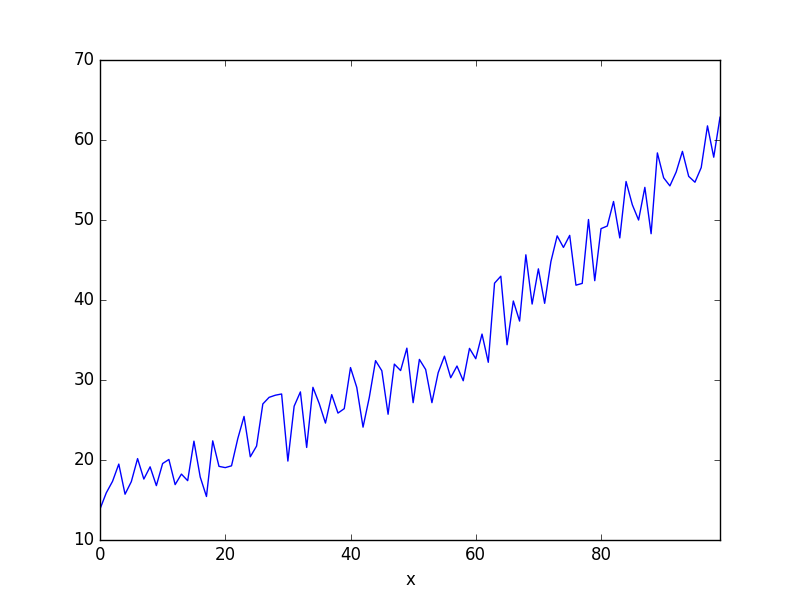
\includegraphics[width=20em]{compscieng_app20_07.png}

Bulunan katsayılar üstteki grafiğe uyuyor. 

İlmik Seçmek

[1, sf. 65] bu tekniği bir adım ilerletiyor; eğer ilmik seçmek isteseydik
ne yapardık? Bu durumda üstteki gibi pek çok mümkün bazı regresyona
verirdik, ama bu sefer regülarizasyon üzerinden eğer ise yaramayanları
cezalandırırsak, çok küçülen katsayılar bizim için önemsiz sayılacaktır ve
katsayısı yüksek olanlar elde tutulabilir. Regularizasyon icin {\em
  Istatistik, Regresyon, Ridge, Lasso, Çapraz Sağlama, Regularize Etmek}.

[1]'in cezalandırma formülasyonu bize bir Ridge regresyonu veriyor. Alttaki
veride denedik,

\begin{minted}[fontsize=\footnotesize]{python}
import pandas as pd
df = pd.read_csv('../../tser/tser_chgpt/cave.csv')
df.C.plot()
plt.savefig('compscieng_app20_06.png')
\end{minted}

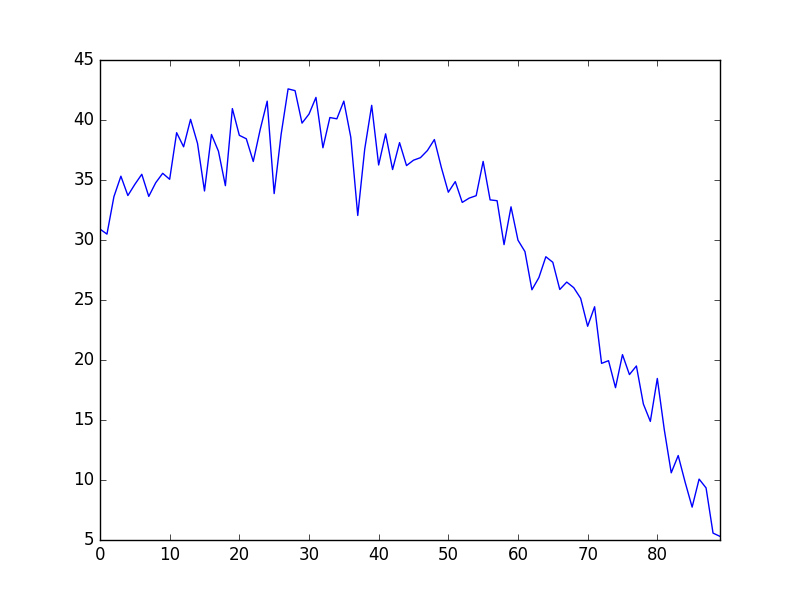
\includegraphics[height=6cm]{compscieng_app20_06.png}

\begin{minted}[fontsize=\footnotesize]{python}
import statsmodels.formula.api as sm
f = "C ~ 1 + Temp + I((Temp > 10)*(Temp-10)) + I((Temp > 15)*(Temp-15)) +" + \
    "I((Temp > 20)*(Temp-20)) + I((Temp > 25)*(Temp-25)) +" + \
    "I((Temp > 30)*(Temp-30)) + I((Temp > 35)*(Temp-35)) +" + \
    "I((Temp > 40)*(Temp-40)) + I((Temp > 45)*(Temp-45)) +" + \
    "I((Temp > 50)*(Temp-50)) + I((Temp > 55)*(Temp-55)) " 
model = sm.ols(formula=f, data=df).fit_regularized(L1_wt=0.0)
print model.summary()
\end{minted}

\begin{verbatim}
                            OLS Regression Results                            
==============================================================================
Dep. Variable:                      C   R-squared:                       0.962
Model:                            OLS   Adj. R-squared:                  0.956
Method:                 Least Squares   F-statistic:                     177.4
Date:                Thu, 12 Jan 2017   Prob (F-statistic):           2.03e-50
Time:                        13:13:45   Log-Likelihood:                -185.82
No. Observations:                  90   AIC:                             395.6
Df Residuals:                      78   BIC:                             425.6
Df Model:                          11                                         
Covariance Type:            nonrobust                                         
================================================================================================
                                   coef    std err          t      P>|t|      [95.0% Conf. Int.]
------------------------------------------------------------------------------------------------
Intercept                       31.8192      1.354     23.494      0.000        29.123    34.515
Temp                             0.3800      0.204      1.863      0.066        -0.026     0.786
I((Temp > 10) * (Temp - 10))    -0.0764      0.497     -0.154      0.878        -1.065     0.912
I((Temp > 15) * (Temp - 15))    -0.0524      0.651     -0.081      0.936        -1.348     1.243
I((Temp > 20) * (Temp - 20))    -0.0027      0.673     -0.004      0.997        -1.342     1.337
I((Temp > 25) * (Temp - 25))    -0.1210      0.674     -0.179      0.858        -1.463     1.221
I((Temp > 30) * (Temp - 30))    -0.3380      0.674     -0.501      0.618        -1.681     1.005
I((Temp > 35) * (Temp - 35))    -0.0869      0.674     -0.129      0.898        -1.429     1.256
I((Temp > 40) * (Temp - 40))     0.1147      0.674      0.170      0.865        -1.227     1.457
I((Temp > 45) * (Temp - 45))     0.0320      0.670      0.048      0.962        -1.302     1.366
I((Temp > 50) * (Temp - 50))    -0.0149      0.598     -0.025      0.980        -1.205     1.176
I((Temp > 55) * (Temp - 55))    -0.6336      0.295     -2.144      0.035        -1.222    -0.045
==============================================================================
Omnibus:                        7.572   Durbin-Watson:                   1.924
Prob(Omnibus):                  0.023   Jarque-Bera (JB):                7.180
Skew:                          -0.575   Prob(JB):                       0.0276
Kurtosis:                       3.770   Cond. No.                         691.
==============================================================================

Warnings:
[1] Standard Errors assume that the covariance matrix of the errors is correctly specified.
\end{verbatim}

İstatistiki modelleri irdelemek bilimden ziyada biraz sanattır, fakat
üstteki sonuçlarda (Temp-30) katsayısının mutlak değerinin orta bölgedeki
diğerlerine göre daha yüksek olduğunu görüyoruz. Grafiğe bakılınca bu
mantıklı gözüküyor.


Alternatif İlmik İfadeleri

Bazen sayısal hesaplarda üstte gördüğümüz $u_+$ ifadesinin $\max(0,x-a)$
ile formülize edildiğini görüyoruz. Yani, 

$$
y = \beta_0 + \beta_1 x + \beta_{2}(x-a)_+ +  \beta_{3}(x-b)_+ + ...
$$

yerine

$$
y = \beta_0 + \beta_1 x + \beta_{2}\max(0,x-a) +  \beta_{3}\max(0,x-b) + ...
$$

ki $a,b$ ilmik noktaları. Bu kullanım da aynı sonuç veriyor, düşünürsek
$\max$ ifadesi $x$ değeri $a$ değerini geçinceye kadar 0, ondan sonra $x-a$
verecek, bu da $u_+$ gibi bir kullanım ile aynı.

Mesela

\begin{minted}[fontsize=\footnotesize]{python}
a,b,c,d = (1, -1.4, 2, 2.5)
x = np.linspace(0,5,100)
knots = [2,3,4]
def f(x):
    return a + \
           b*np.max([0,x-knots[0]]) + \
           c*np.max([0,x-knots[1]]) + \
           d*np.max([0,x-knots[2]])
	   
    
y = np.array([f(xx) for xx in x])
plt.plot(x,y,'.')
plt.savefig('compscieng_app20_10.png')
\end{minted}

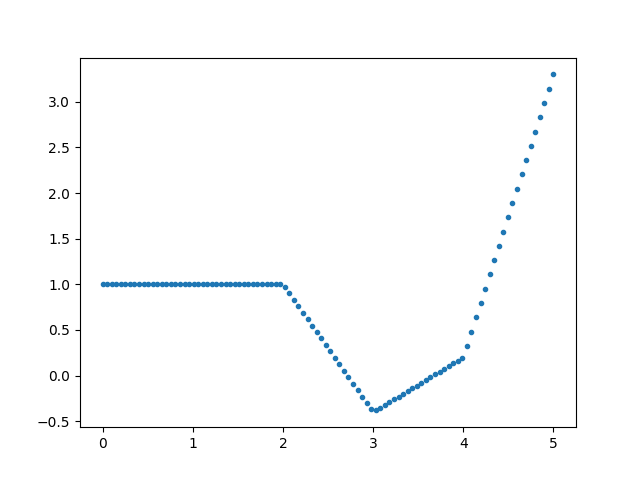
\includegraphics[width=20em]{compscieng_app20_10.png}

Rasgele bazı ağırlıklarla $x=2,3,4$ noktalarında aktif olan ilmiklerle
üstteki grafiği çıkarttık. Regresyon bağlamında bir optimizasyon rutinine
(illa lineer regresyon olması gerekmez) veriye bakarak bir hatanın minimize
edilmesi üzerinden en optimal $a,b,c,d$ ağırlıklarını buldurmak ta
mümkündür. 

Peki $\max$ yerine baska bir fonksiyon kullanabilir miydik? $\max$'in
sonucta yaptigi belli bir esik degerinden once 0 sonrasinda baska bir deger
vermek degil midir? Evet. Bu tur bir ``karar'' fonksiyonu sigmoid ile de
elde edilebilir. 

\begin{minted}[fontsize=\footnotesize]{python}
alpha = 5.0
def sig(x,a):
   return 1/(1+np.exp(-alpha*(x-a)))
x = np.linspace(-5,5,100)
\end{minted}

\begin{minted}[fontsize=\footnotesize]{python}
y = sig(x,0)
plt.plot(x,y)
plt.savefig('compscieng_app20_11.png')
\end{minted}

\begin{minted}[fontsize=\footnotesize]{python}
y = sig(x,3)
plt.plot(x,y)
plt.savefig('compscieng_app20_12.png')
\end{minted}

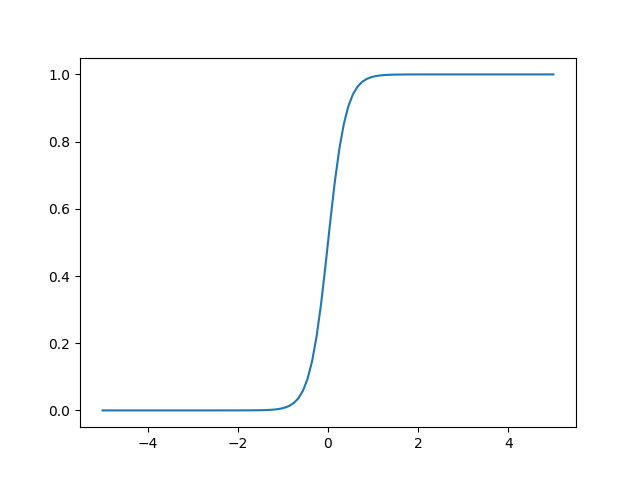
\includegraphics[width=20em]{compscieng_app20_11.png}
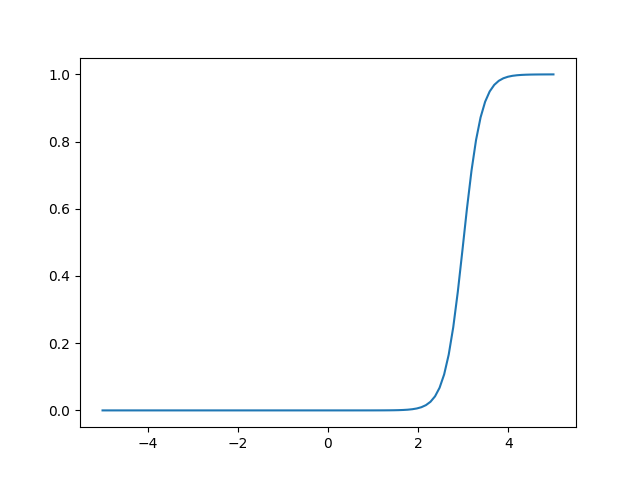
\includegraphics[width=20em]{compscieng_app20_12.png}

Normal sigmoid üst soldaki, fakat $x-a$ ile onu da istediğimiz noktaya
kaydırabiliyoruz. $\alpha$ parametresi 0'dan 1'e geçişin ne kadar sert
olduğunu kontrol ediyor.

\begin{minted}[fontsize=\footnotesize]{python}
rho = 7.0
def sig2(x,a):
   return (x-a)*1/(1+np.exp(-rho*(x-a)))

a,b,c,d = (1, -1.4, 2, 2.5)
x = np.linspace(0,5,100)
knots = [2,3,4]
def f(x):
    return a + \
           b*sig2(x,knots[0]) + \
           c*sig2(x,knots[1]) + \
           d*sig2(x,knots[2])
	       
y = np.array([f(xx) for xx in x])
plt.plot(x,y)
plt.savefig('compscieng_app20_13.png')
\end{minted}

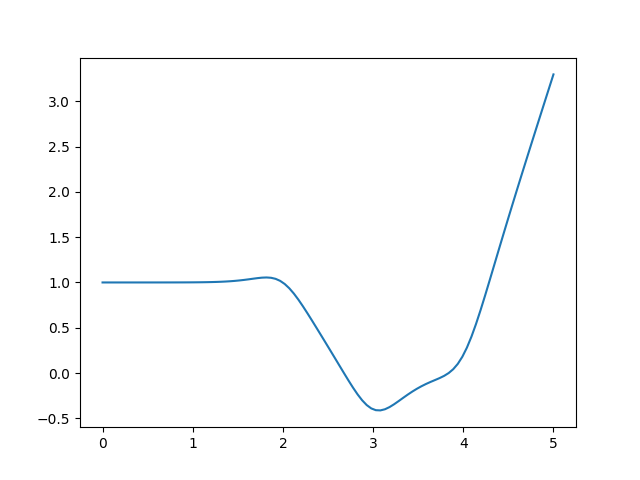
\includegraphics[width=20em]{compscieng_app20_13.png}

Daha yumuşak, pürüzsüz bir fonksiyon elde etmiş olduk. Bu birleşik eğrinin
türevini almak ta daha kolay olacaktır. Gerçi otomatik türev paketleri
artık içinde $\max$ bile olan ifadelerin türevini alabiliyor, fakat
üsttekinin sembolik türevi rahatça alınabilir, bu seçeneğin elde olması iyidir.

Küpsel Spline Eğrileri (Cubic Splines)

Baz seçerken elimizde pek çok seçenek var, mesela küpsel spline eğrileri
uydurmak için

$$ (1,x,x^2,x^3,(x-k_1)_+^3,(x-k_2)_+^3,(x-k_3)_+^3,.. )$$

gibi bir baz kullanabiliriz, ilmikler $k_1,..,k_K$ olarak gider, genel
olarak

$$ f(x) = \beta_0 + \beta_1x + \beta_2 x^2 + \beta_3 x^3 + 
\sum_{s=1}^{K} \beta_{3+s} (x-k_s)^3_+
$$

formülü verilir. Bu baza kırpılmış güç bazı (truncated power basis) ismi de
veriliyor. 

Bir örnek üzerinde görelim,

\begin{minted}[fontsize=\footnotesize]{python}
import pandas as pd
dfcube = pd.read_csv('cube.csv')
df2 = dfcube.set_index('x')
df2.y.plot()
plt.savefig('compscieng_app20_09.png')
\end{minted}

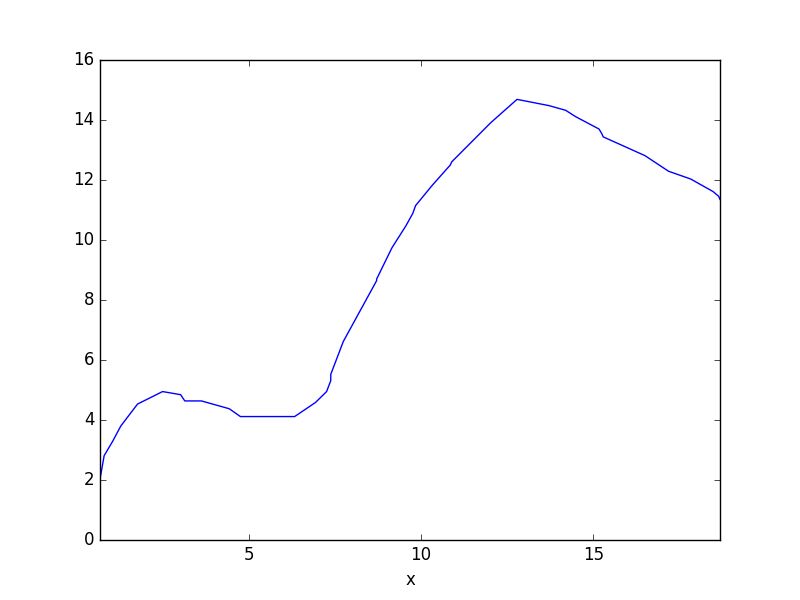
\includegraphics[width=20em]{compscieng_app20_09.png}

İlmik noktalarını seçelim, 8 ve 13 noktasında olsun,

\begin{minted}[fontsize=\footnotesize]{python}
import pandas as pd
import statsmodels.api as sm

dfcube = pd.read_csv('cube.csv')
dfcube.loc[:,'1'] = 1.
dfcube.loc[:,'x2'] = dfcube.x**2
dfcube.loc[:,'x3'] = dfcube.x**3
k1 = dfcube.x-8; dfcube.loc[k1>0,'k1'] = k1**3
k2 = dfcube.x-13; dfcube.loc[k2>0,'k2'] = k2**3
dfcube = dfcube.fillna(0)
X = dfcube[['1','x','x2','x3','k1','k2']]
y = dfcube.y
f = sm.OLS(y,X).fit()
print f.params
\end{minted}

\begin{verbatim}
1     1.586781
x     1.747705
x2   -0.381304
x3    0.030443
k1   -0.092883
k2    0.138559
dtype: float64
\end{verbatim}

\begin{minted}[fontsize=\footnotesize]{python}
dfcube['yy'] = f.params[0]*dfcube['1'] + f.params[1]*dfcube.x + \
               f.params[2]*dfcube.x2 + f.params[3]*dfcube.x3 + \
               f.params[4]*dfcube.k1 + f.params[5]*dfcube.k2 
dfcube['y'] = y
df2 = dfcube.set_index('x')
df2[['y','yy']].plot()
plt.hold(True)
plt.axvline(x=8,color='c')
plt.hold(True)
plt.axvline(x=13,color='c')
plt.savefig('compscieng_app20_08.png')
\end{minted}

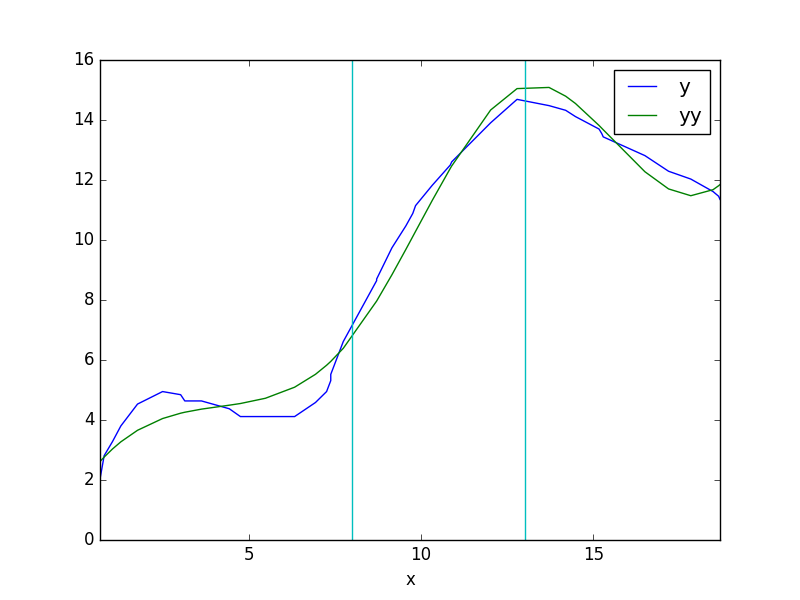
\includegraphics[width=20em]{compscieng_app20_08.png}

Kısıtlanmış Küpsel Spline Eğrileri (Restricted Cubic Splines)

Üstteki metot iyi işliyor, fakat bazen başta ve sondaki parçaların eğri
değil tam düz olması istenebiliyor, yani ``eteklerde'' düzleştirme
amaçlanıyor. Bu özel formülasyon için bkz. [3, sf. 24]. Bu yaklaşımı baz
alan kod [1]'in Python çevrimini altta veriyoruz. Metota verilen isim
kısıtlanmış küpsel spline eğrileri, ya da doğal spline eğrileri (natural
splines). 

\begin{minted}[fontsize=\footnotesize]{python}
import scipy.linalg as lin

def rcs(x,y,knots):
    n = len(y)
    k = knots
    X1 = x
    q = len(k)-1
    myX=np.zeros((n,len(knots)-2))

    for j in range(q-1):
    	tmp1 = (x-k[j])**3 * (x>k[j])
	tmp2 = (x-k[q-1])**3 * (x>k[q-1])*(k[q]-k[j])
	XX= tmp1-tmp2/(k[q]-k[q-1])
        tmp1 = (x-k[q])**3 * (x>k[q])
        tmp2 = (k[q-1]-k[j])
	XX = XX+tmp1*tmp2/(k[q]-k[q-1])
	myX[:,j]=XX

    X = np.hstack( (np.ones((n,1)),np.reshape(X1,(n,1)),myX) )
    bhat = np.linalg.lstsq(X,y)[0]
    bhatt = np.zeros(len(knots)+1)
    bhatt[len(bhat)] = (bhat[2:]*(k[0:-2]-k[-1])).sum()
    bhatt[len(bhat)] = bhatt[len(bhat)] / (k[-1]-k[-2])
    bhatt = np.hstack([bhatt, 0])    
    bhatt[-1] = (bhat[2:]*(k[0:-2]-k[-2])).sum()
    bhatt[-1] = bhatt[-1] / (k[-2]-k[-1])
    bhat = np.hstack((bhat, bhatt[-2:]))
    return bhat

def speval(x,coefs,knots):
    tmp = coefs[0] + coefs[1]*x 
    for k in range(len(knots)): 
         tmp = tmp + coefs[k+2]*((x-knots[k])**3)*(x>knots[k])
    return tmp
\end{minted}


\begin{minted}[fontsize=\footnotesize]{python}
import pandas as pd
x = np.random.randn(300)*np.sqrt(2)
e = np.random.randn(300)*np.sqrt(0.5)
y = np.sin(x)+e
df = pd.DataFrame([x,y]).T
df.columns = ['x','y']
df = df.sort_index(by='x')
print df.head()
knots=np.array([-5.5938, -3.7732, -1.9526, -0.1320, 1.6886, 3.5092, 5.3298]);
bhat = rcs(df.x,df.y,knots)
print bhat
df['spline'] = speval(df.x, bhat, knots)
df2 = df.set_index('x')
df2[['y','spline']].plot()
plt.hold(True)
for k in knots: plt.plot(k,speval(k,bhat,knots),'rd')
plt.savefig('compscieng_app20_01.png')
\end{minted}

\begin{verbatim}
            x         y
156 -4.037867  0.786392
214 -3.442141  0.716684
101 -3.331777  0.400504
249 -3.178510 -1.019875
235 -3.131058  0.309575
[ 2.60209869  0.37061018 -0.09614395  0.3059325  -0.30256291 -0.05312331
  0.33303297 -0.24924314  0.06210785]
\end{verbatim}

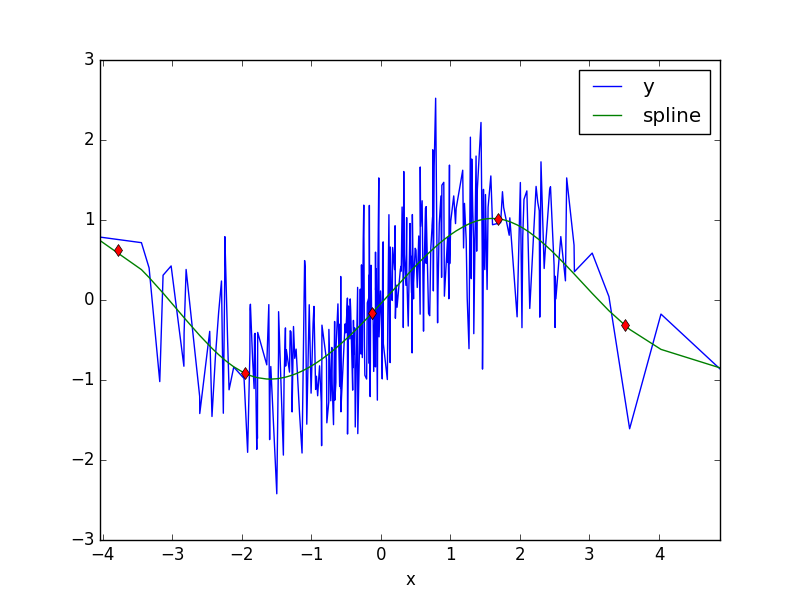
\includegraphics[width=20em]{compscieng_app20_01.png}

\begin{minted}[fontsize=\footnotesize]{python}
import pandas as pd
dfcube = pd.read_csv('cube.csv')
dfcube = dfcube.sort_index(by='x')
knots=np.array([3,5,8,14,14.5]);
bhat = rcs(dfcube.x,dfcube.y,knots)
print bhat
dfcube['spline'] = speval(dfcube.x, bhat, knots)
df2 = dfcube.set_index('x')
df2[['y','spline']].plot()
plt.hold(True)
for k in knots: plt.plot(k,speval(k,bhat,knots),'rd')
plt.savefig('compscieng_app20_03.png')
\end{minted}

\begin{verbatim}
[ 3.16368016  0.17418578  0.02336622 -0.01432746 -0.05277535  0.42087813
 -0.37714154]
\end{verbatim}

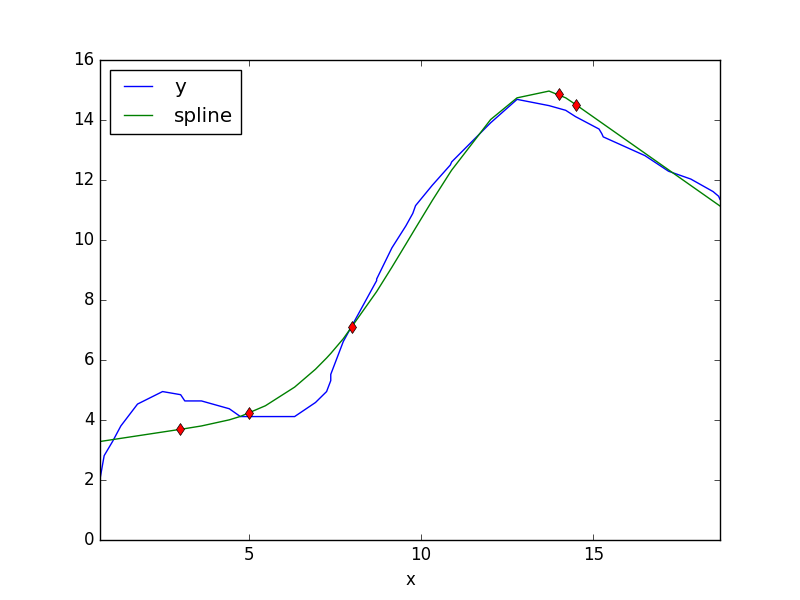
\includegraphics[width=20em]{compscieng_app20_03.png}


Kaynaklar

[1] Bantis, {\em Restricted Cubic Spline}, \url{https://uk.mathworks.com/matlabcentral/fileexchange/41241-restricted-cubic-spline}

[2] Ruppert, {\em Semiparametric Regression}

[3] Harrell, {\em Regression Modeling Strategies, 2nd Edition}

[4] Bayramlı, Lineer Cebir, {\em Ders 16}

[5] Bayramlı, İstatistik, {\em Lineer Regresyon}



\end{document}
